% !TeX encoding = UTF-8
% !TeX program = LuaLaTeX

% 调用模板
% 格式文件
% !TeX encoding = UTF-8
% !TeX program = LuaLaTeX

%%% 设置页面布局
% 设置页边距
\usepackage{geometry}
% 设置缩进
\setlength{\parindent}{0pt}
% 设置段落间距
\setlength{\parskip}{1.5em}
% 设置颜色
\usepackage{color}

% 删除线插件
\usepackage[normalem]{ulem}
% 插图插件
\usepackage{graphicx}

% 设置自定义列表图标
% 自定义星星图标
\newcommand{\parStar}{%
    \par\noindent
    \smash{%
    \makebox[0pt]{%
    \raisebox{\dimexpr-.5\height+.3\baselineskip}{%
    
\includegraphics[height=10pt]{itemStar.png}%
      }%
    }%
  }%
  \hspace*{\parindent}}

% 自定义星球图标
\newcommand{\parPlant}{%
    \par\noindent
    \smash{%
    \makebox[0pt]{%
    \raisebox{\dimexpr-.5\height+.3\baselineskip}{%
    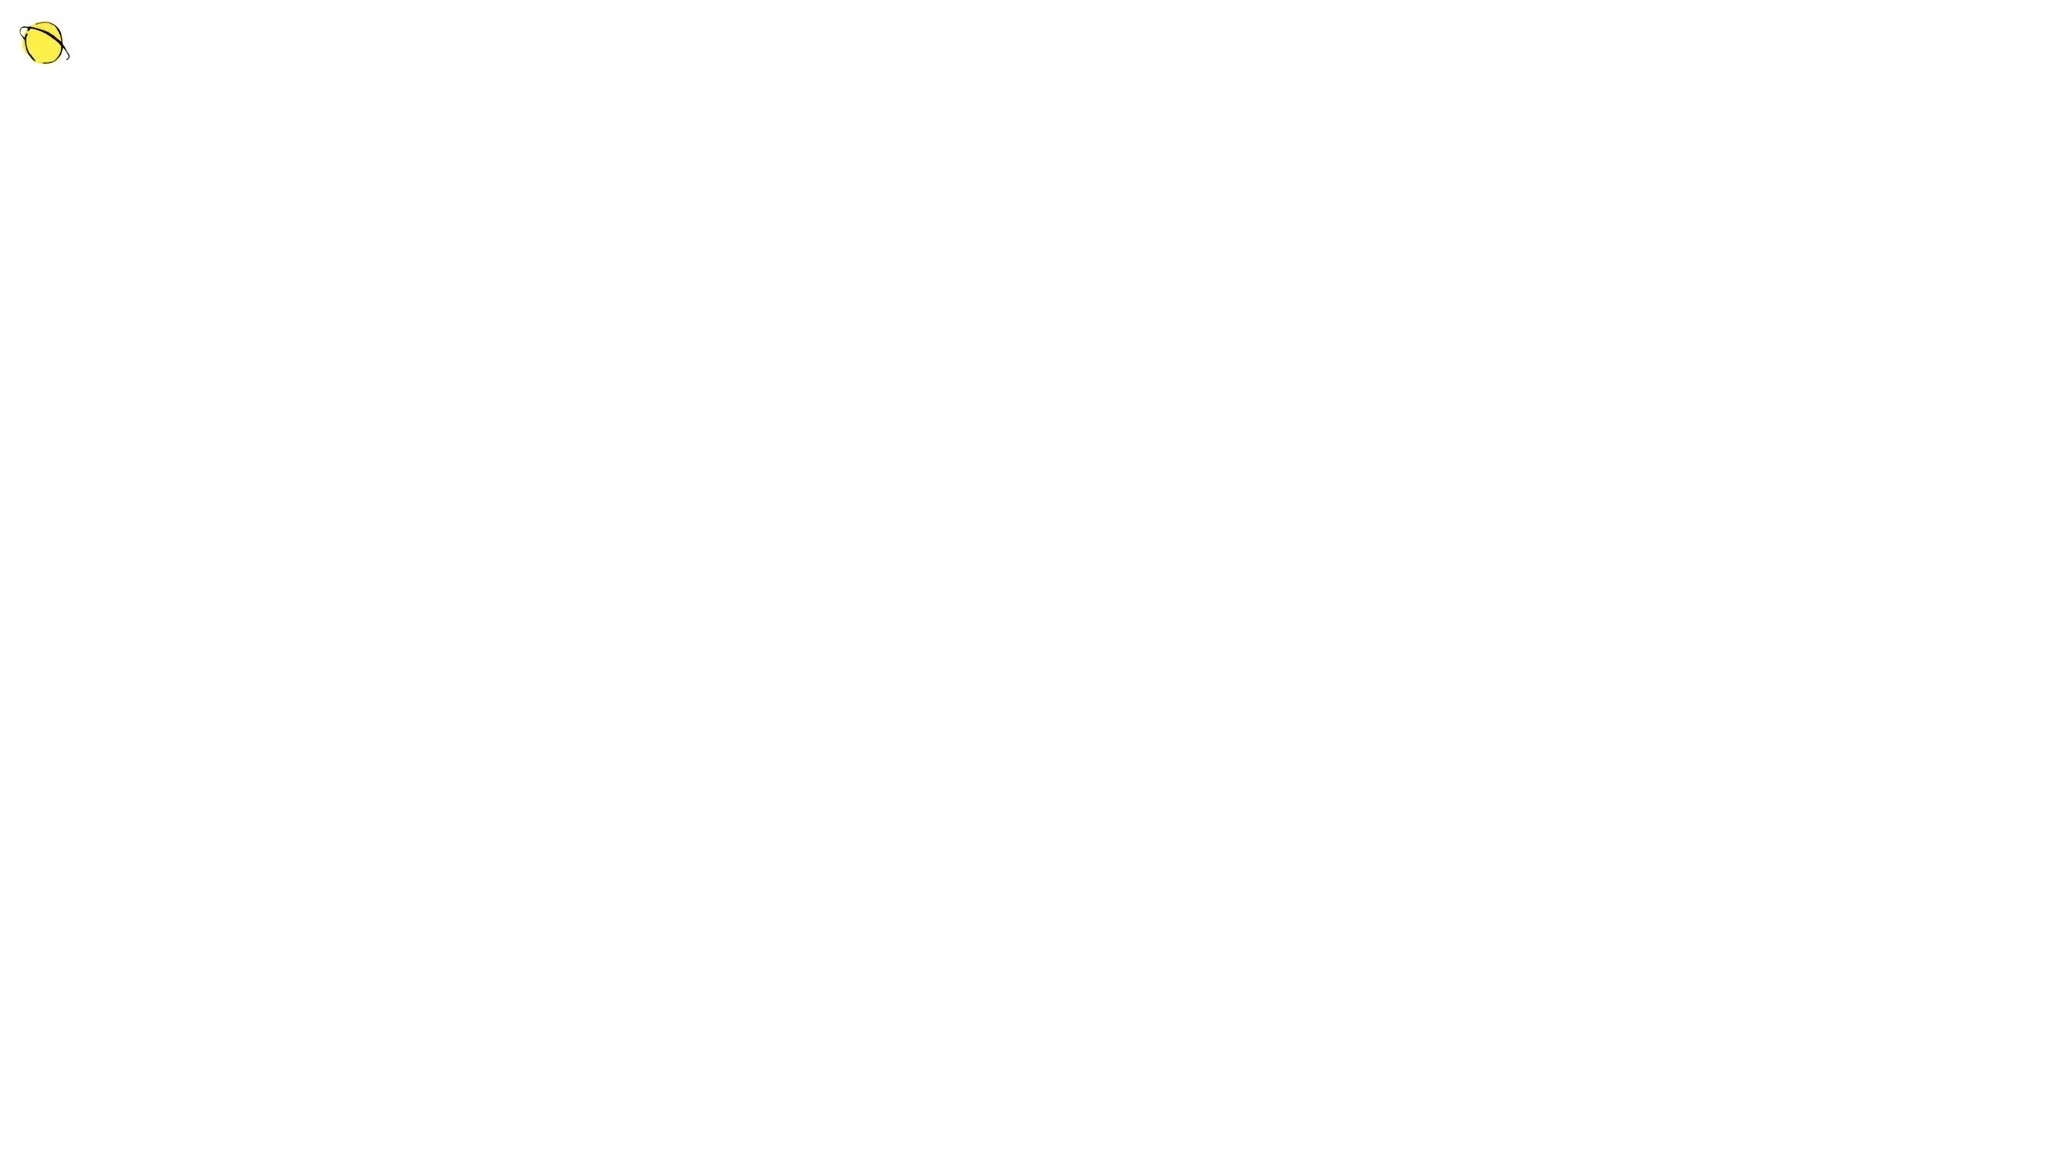
\includegraphics[height=10pt]{itemPlant.png}%
      }%
    }%
  }%
  \hspace*{\parindent}}
  
% 自定义野花图标
\newcommand{\parFlw}{%
    \par\noindent
    \smash{%
    \makebox[0pt]{%
    \raisebox{\dimexpr-.5\height+.3\baselineskip}{%
    
\includegraphics[height=10pt]{itemFlw.png}%
      }%
    }%
  }%
  \hspace*{\parindent}}
%%% CJK language setting

%%% xeCJK package under XeTeX, suitable for Chinese doc
% \usepackage[space]{xeCJK}
%% Chinese as the main language
% \setCJKmainfont{Noto Serif CJK SC}
% \setCJKsansfont{Noto Sans CJK SC}

%% Define fonts for Japanese and Korean
% \newCJKfontfamily\japanesefont{Noto Serif CJK JP}

%%% LuaTexja package under LuaTeX, suitable for Japanese doc
\usepackage{luatexja}            % Basic package
\usepackage{luatexja-ruby}       % 调用振假名插件
\ltjsetruby{size=0.6}            % 设置振假名字号
%\ltjsetruby{fontcmd=\gtfamily}  % 设置振假名字体
\ltjsetruby{mode=00}             % 设置振假名的「進入」和「突出」模式

%\usepackage{pxrubrica}          % 同为振假名插件

\usepackage{luatexja-fontspec}   % 字体设置插件
% 为了实现中日双语混排,需要调用中文字体
\setmainjfont{SIMSUN.TTC}[AutoFakeBold]        % 调用嵌入的简体宋体

% 修改页眉页脚默认字体
\usepackage{fancyhdr}
\newcommand{\cjkfont}{%
\fontfamily{SIMSUN.TTC}\fontseries{b}\fontsize{9}{11}\selectfont}
% 定义页眉页脚使用的文档部件
\usepackage{titlesec}
\renewcommand{\sectionmark}[1]{%
\markboth{#1}{}}

%%% 其他工具包
% 自定义章节名称插件
\usepackage{titlesec}
% 页码格式
\usepackage{inputenc}

% 网页超链接插件
\usepackage{hyperref}
% 超链接高亮颜色设置
% 加载色彩工具包
\usepackage[svgnames]{xcolor}
% 自定义色彩
\definecolor{VolcanoGray}{RGB}{147, 159, 174}
\definecolor{RossRed}{RGB}{146, 71, 62}
\definecolor{Baobab}{RGB}{120, 140, 97}
\definecolor{FoxOrange}{RGB}{239, 171, 93}
\definecolor{ClothGreen}{RGB}{159, 174, 166}
\definecolor{SmokeBlue}{RGB}{79, 129, 155}
% 色彩调用-超链接文本
\hypersetup{
    colorlinks=true,
    linkcolor=SmokeBlue,
    filecolor=RossRed,      
    urlcolor=SmokeBlue,
}
% 色彩调用-页边注(sidenote有编号,marginnote无编号)
\setsidenotefont{\color{VolcanoGray}\footnotesize}
\setmarginnotefont{\color{VolcanoGray}\footnotesize}

% Spacing setting
\large
\selectfont

% Date in Chinese
\renewcommand{\today}{\number\year 年 \number\month 月 \number\day 日}




%%% Title and author information
\title[「星の王子さま」]{「星の王子さま」日语学习笔记}
\author{By-是我 \sout{Dio} Qu哒
\thanks{只是我无聊的玩梗}}

\begin{document}
  \maketitle

% 自定义页眉页脚
% 此处默认双面布局
\thispagestyle{plain}
\fancyhead[LO,RE]{「星の王子さま」日语学习笔记}
\fancyhead[LE,RO]{写在前面}
\fancyfoot[C]{\thepage}
\pagenumbering{roman}

\section*{\bf{Hi! 很高兴见到你!}}
这份资料是以《小王子》为基础整理的文型、单字笔记。笔记的排版是之前上课的习题排版,左边是日文,右边是中文翻译、注释和碎碎念。感觉「星の王子さま」的译名还是要比「 あのときの王子くん 」亲切,姑且就先这样吧。如果这一版制作顺利的话,下一本想讲《银河铁道之夜》,广播剧和85版动画都好喜欢\marginnote{这版才刚开个头就在想些有的没的}。

因为现在自己也才刚入门,笔记应该会涉及很多基础知识点。不过五十音拼读还是需要的,有关五十音的入门介绍会整理在附录里。如果出现汉字,笔记里会注上假名。青空这版电子书99\%都是假名,作为学习材料,笔记里也会尽量注上汉字。

\section*{\bf{学习资料传送}}

    \parStar \href{https://www.aozora.gr.jp/cards/001265/files/46817_24670.html}{日版《小王子》电子书}, 收录于青空文库({ 青空文庫})电子图书馆。大量已经公开版权的日文作品都可以在这里找到。
    
    \parStar \href{https://music.163.com/#/album?id=3139032}{「星の王子さま」广播剧},这一辑是在原文基础上分角色演绎的版本。可能因为译者不同,和青空文库的版本不完全一致\marginnote{这下不知道该着手哪个版本才好了},但网友有配上滚动字幕和翻译。
    
    \parStar 日本老师用中文讲解日语的系列,是目前看到最适合零基础入门的教程=)50p的文法课也没有很枯燥,有配套教程但目前只看视频也还好。小说整理出来的知识点更多只是把联系变得 有意思\marginnote{日剧、日漫、综艺和日文歌都是如此},扎实的语法还是需要系统化的教程呐。
    \begin{itemize}
        \setlength\itemsep{0.5em}
        
        \item \href{https://www.bilibili.com/video/BV1mt411M7Uy/?p=6}{五十音入门-B站} / \href{https://www.youtube.com/playlist?list=PLynCeSdpMqxBipKl9EHnBzZFzBnGuB108}{油管}
        
        \item \href{https://www.bilibili.com/video/BV1NJ41187DK?t=48}{出口日语文法教程-B站} / \href{https://www.youtube.com/playlist?list=PLynCeSdpMqxCW-AfMtmIlASAMUVq8wX6k}{油管}
        
    \end{itemize}
    
    \parStar 在线日文词典工具箱\marginnote{目前还只是跟着视频学语法,这部分之后慢慢补充上来}
    \begin{itemize}
        \setlength\itemsep{0.5em}
        
        \item \href{https://cjjc.weblio.jp/}{Weblio日中/中日词典}
        
        \item 移动端上的手写词典应用「白檜辞書」(Shirabe Jisho),适合查不认识的单字发音
    \end{itemize}
    
    \parStar 日文输入法的话,推荐\href{https://www.google.co.jp/ime/}{Google日文输入法} \marginnote{学校的电脑上没有管理员权限,Google输入法总是安装失败。微软自带的输入法几乎不能输入假名,完全是用不上的屑,可能也有权限问题啦。Mac自带的输入法好像就还可以用。}。Chrome上也有\href{https://chrome.google.com/webstore/detail/google-input-tools/mclkkofklkfljcocdinagocijmpgbhab/related}{Google Input Tools}插件支持罗马音和手写输入,查单词、敲课文完全可以。

%%% 开始正文
\newpage
\pagenumbering{arabic}
\setcounter{page}{1}

% 双面布局页眉
\fancypagestyle{plain}
\fancyhf{} % clear all header and footer fields
\fancyhead[LO,RE]{「星の王子さま」日语学习笔记}
\fancyhead[LE,RO]{\leftmark}
\fancyfoot[C]{\thepage}

%%% 第一章 %%%
\section{1}
ぼくが6つのとき、よんだ本にすばらしい絵があった。『ぜんぶほんとのはなし』という名まえの、しぜんのままの森について書かれた本で、そこに、ボアという大きなヘビがケモノをまるのみしようとするところがえがかれていたんだ。だいたいこういう絵だった。

\begin{figure}
    \centering
    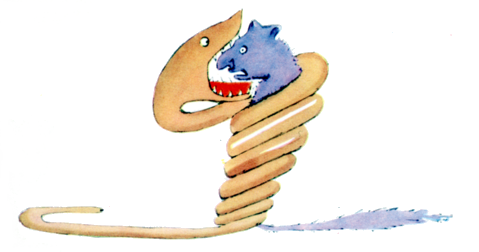
\includegraphics{fig46817_02.png}
\end{figure}



%%% 附录部分
\newpage
\setcounter{page}{1}
%\setcounter{section}{1}

% 双面布局页眉
\fancyhf{} % clear all header and footer fields
\fancyhead[LO,RE]{附录 \thesection}
\fancyhead[LE,RO]{\leftmark}
\fancyfoot[C]{\thepage}
\pagenumbering{Roman}

\section{五十音}
五十音书写和发音应该是最最基本的要点了吧~
知道汉字起源后,对平片假名印象会更深
我在看视频的时候有反复抄写,之后学单词、文法都会不断加深印象,所以感觉不用特别花时间再去死记硬背
刚开始容易记混时,有用便利贴写上4、5个平片假名,零零星星贴在厕所镜子、窗边、冰箱门这种存在感高的地方,偶尔瞄到提醒一下。

\newpage
\section{动词结构}

\end{document}